\chapter{Data Assimilation}
\label{var_chap}

An introduction to the basic ideas of variational data assimilation and
the WRF Data Assimilation (WRFDA) system \citep{barker12} is given in this chapter, followed by a brief
overview of recent major improvements to WRFDA.  This overview
supplements the original description of the three-dimensional
variational (3D-Var) algorithm found in \citet{barker04} with
several important additions and modifications, including a utility {\it gen$\_$be}
for calculating background error covariances, several new data assimilation algorithms, and
new and improved capabilities to assimilate satellite radiance and radar observations.

\section{Introduction}
\label{var-intro}

The basic goal of any variational data assimilation system is to produce
an optimal estimate of the true atmospheric state at analysis time
through iterative solution of a prescribed cost-function \citep{ide97}:

\begin{equation}
J({\bf x}) = J_b({\bf x}) + J_o({\bf x}) = \frac{1}{2 
} ({\bf x}-{\bf x}^{b})^{T}{\bf B}^{-1}({\bf x}-{\bf x}^{b}) + 
\frac{1}{2}
({\bf y}-{\bf y}^{o})^{T}({\bf E+F})^{-1}({\bf y}-{\bf y}^{o}).
\label{cost_function}
\end{equation}

The variational problem can be summarized as the iterative minimization
of (\ref{cost_function}) to find the analysis state ${\bf x}$ that
minimizes $J({\bf x})$. This solution represents the {\it a posteriori}
maximum likelihood (minimum variance) estimate of the true state of the
atmosphere given the two sources of {\it a priori} data: the first guess
(or background) ${\bf x^{b}}$ and observations ${\bf y^{o}}$
\citep{lorenc86}. The fit to individual data points is weighted by
estimates of their errors: ${\bf B}$, ${\bf E}$, and ${\bf F}$ are the
background, observation (instrumental), and representative error
covariance matrices, respectively. The representative error is an estimate of
inaccuracies introduced via the observation operator $H$ used to
transform the gridded analysis ${\bf x}$ to observation space ${\bf
y}=H({\bf x})$ for comparison against observations. This error will be
resolution dependent and may also include a contribution from
approximations (e.g., linearizations) in $H$.

As described in \citet{barker04}, the particular variational data
assimilation algorithm adopted in WRFDA is a model-space, incremental
formulation of the variational problem.  In this approach, observations,
previous forecasts, their errors, and physical laws are combined to
produce analysis increments ${\bf x^{a'}}$, which are added to the first
guess ${\bf x^{b}}$ to provide an updated analysis.

Figure \ref{var-sketch} illustrates the relationship between WRFDA,
the various datasets, and the other components of a typical NWP system
(here ARW). The WRFDA assimilation proceeds as described in
\citet{barker04}. A number of recent upgrades to the WRFDA algorithm
will be described in Section \ref{var-upgrade}.

%
%  Figure 9.1 var-sketch
%
\begin{figure}
  \centering
  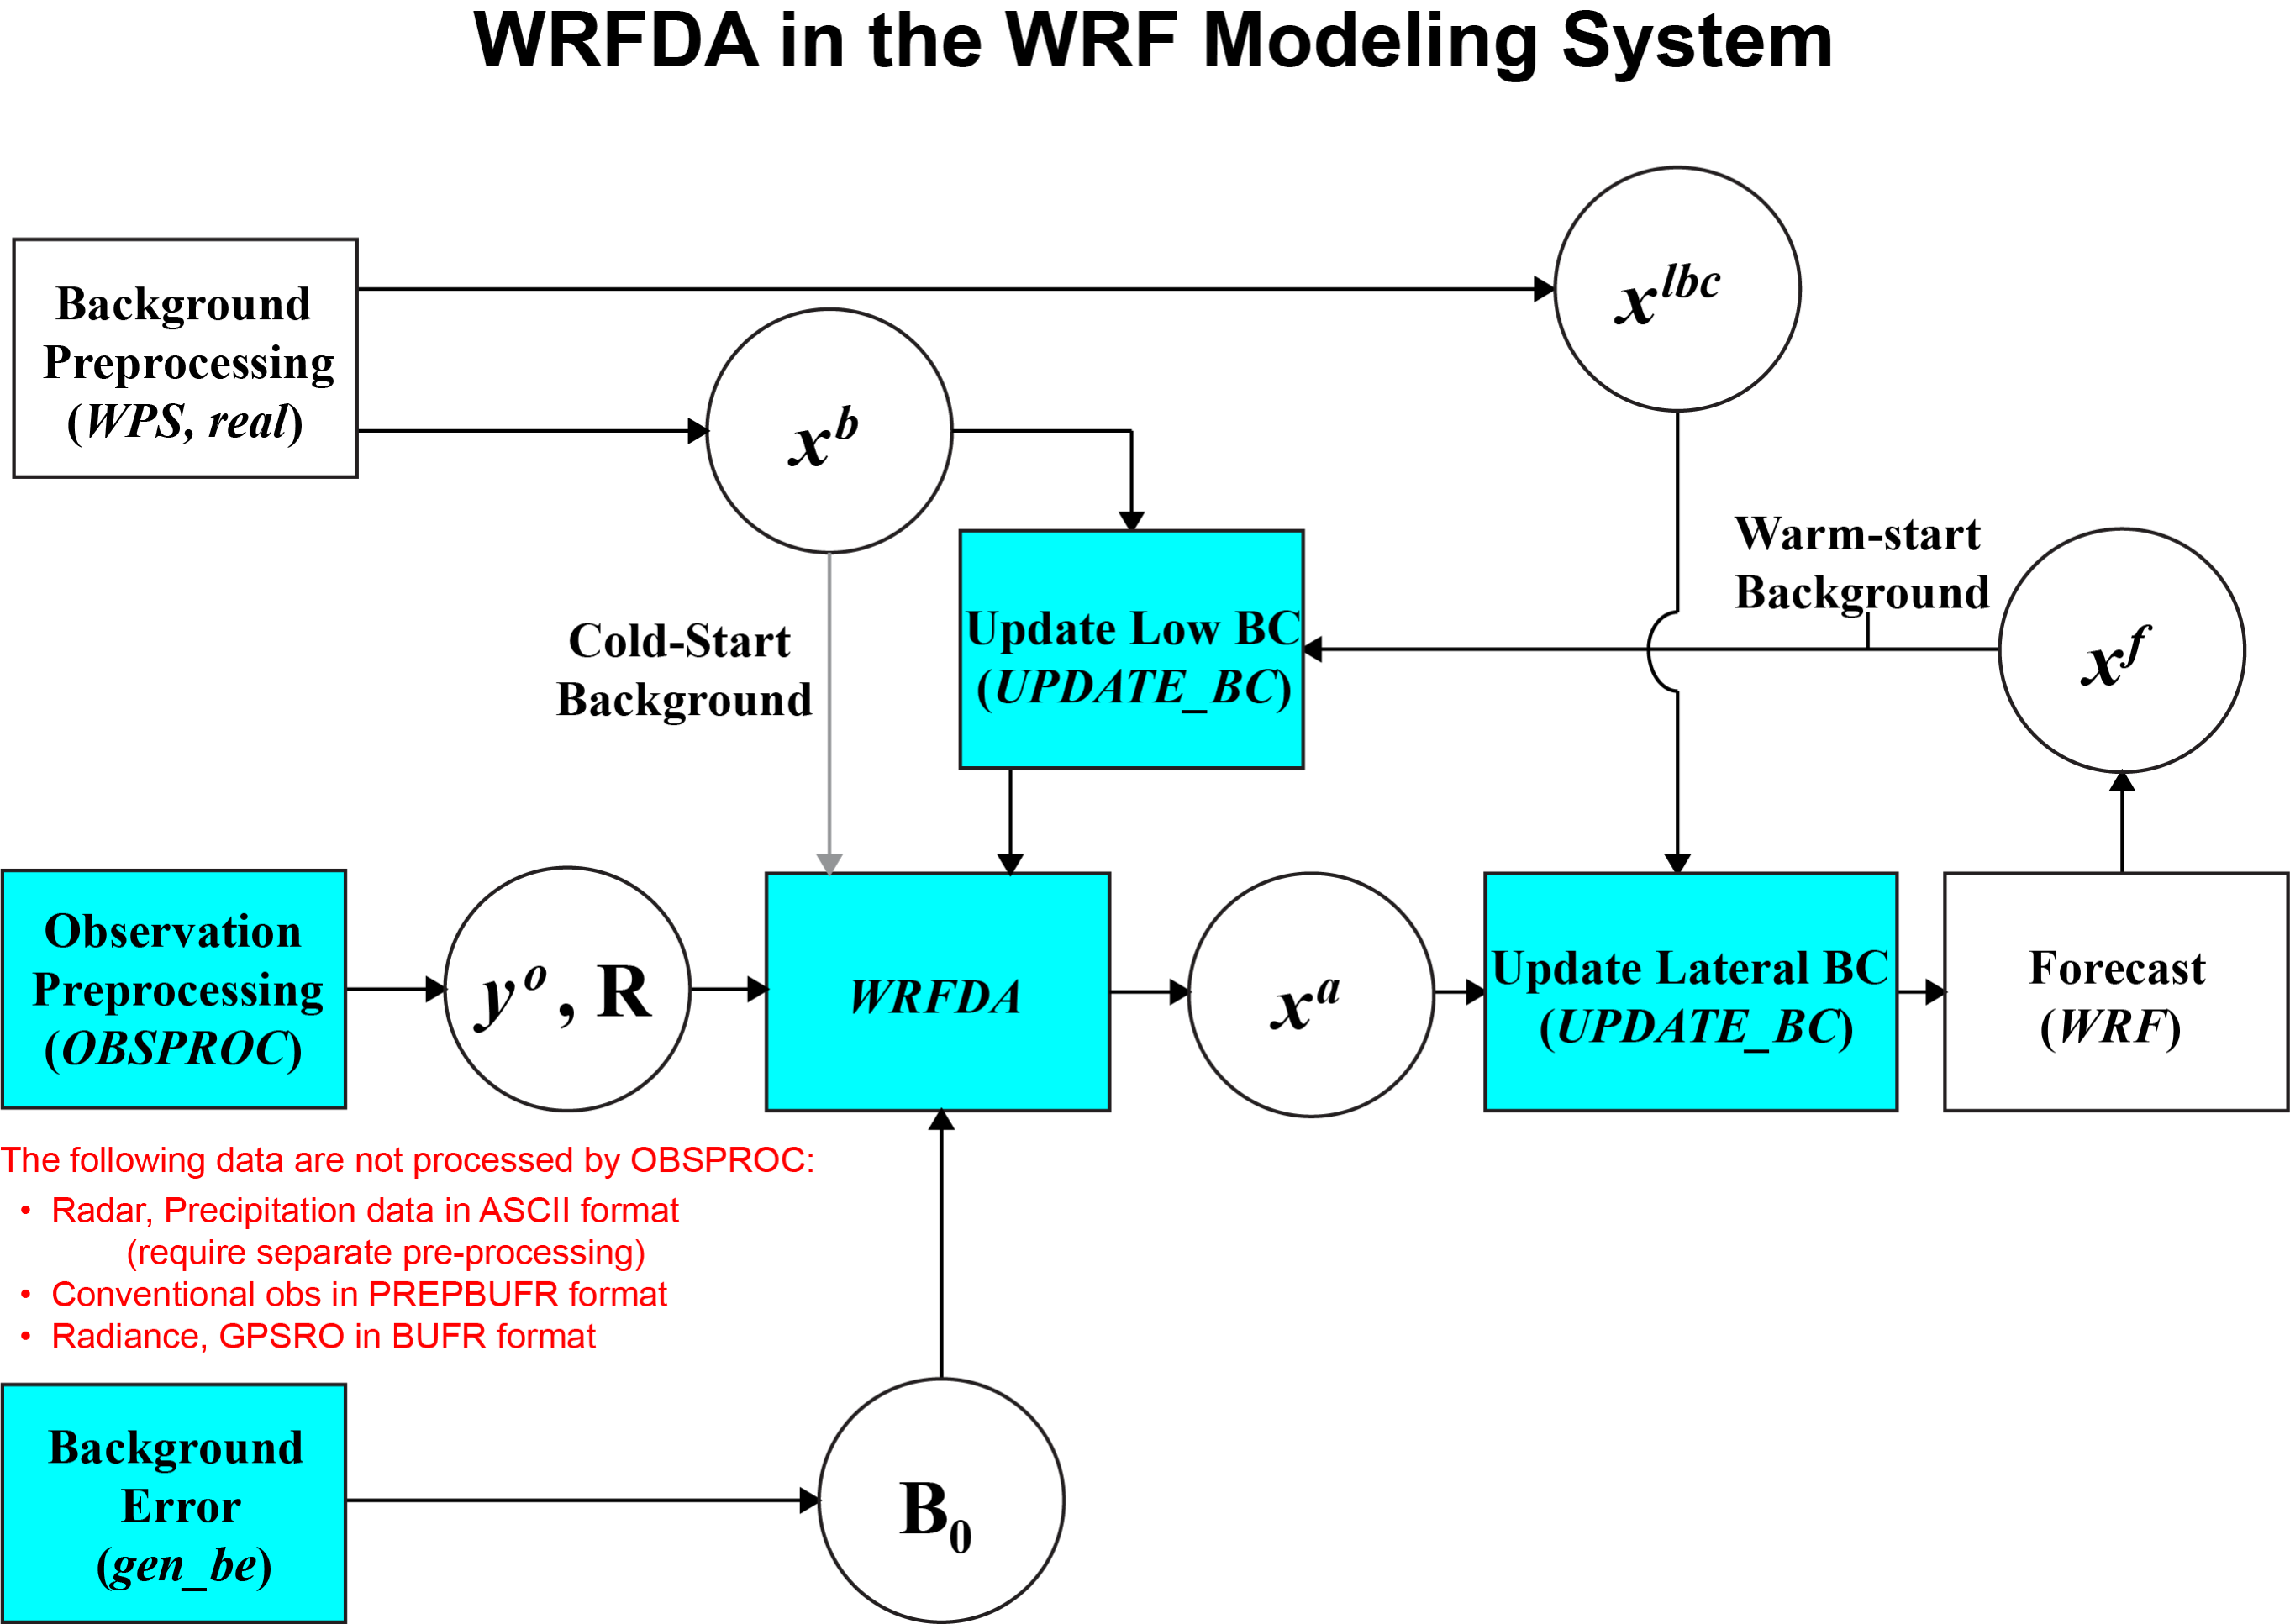
\includegraphics[width=6.5in]{figures/var-sketch.pdf}
  \caption{\label{var-sketch}Sketch showing the relationship between datasets (circles), 
           and algorithms (rectangles) of ARW system.}
\end{figure}

The three inputs to WRFDA are: 

\vspace{0.5cm}

a) First guess ${\bf x^{b}}$--- In cold-start mode, this is typically a
forecast/analysis from another model interpolated to ARW grid (and variables) via the 
WPS and ARW {\it real} programs. In cycling mode, the first guess 
is a short-range (typically 1--6 hour) ARW forecast. 

\vspace{0.5cm}

b) Observations ${\bf y^{o}}$--- In the current version of WRFDA, observations may be 
supplied either in PREPBUFR format ({\it ob\_format=1}) or an ASCII ``little\_r" format
({\it ob\_format=2}). An observation preprocessor (OBSPROC) 
is supplied with the code release to perform basic quality control, assign ``total" 
observation errors (${\bf R = E+F}$ in Fig. \ref{var-sketch}), and reformat observations from the MM5 {\it little$\_$r} text 
format into WRFDA's own text format. Details can be found in \citet{barker03, barker04}.

\vspace{0.5cm}

c) Background error covariances ${\bf B}$--- used to define the spatial
and multivariate response of the analysis to an observation. In
variational systems, these covariances are typically calculated
off-line, and significant tuning is required to optimize performance
for a particular application (e.g., \citet{ingleby01, wu02}). The
amount of work required to do this satisfactorily is significant, and
should not be underestimated. In order to assist the user, the WRFDA
developers supply the following: i) a default set of statistics used
for the initial set up of a domain; ii) a utility {\it gen$\_$be}
(described in Section
\ref{var-be}) to process ensembles of forecasts into the appropriate control variable 
space; and iii) diagnostic routines to assess the accuracy of
observation and background error statistics. These routines include
both innovation vector-based approaches \citep{hollingsworth86} and
variational tuning approaches \citep{desroziers01}.

Following assimilation of all data, an analysis ${\bf x^{a}}$ is produced that must be 
merged with the existing lateral boundary conditions ${\bf x^{lbc}}$ in the {\it UPDATE\_BC} 
utility (\citet{barker03}). At this stage, the {\it wrfbdy} lateral boundary condition 
files (${\bf x^{lbc}}$) output of WPS/real is updated to make the lateral boundaries consistent 
with the analysis, and surface fields (e.g. SST) are also updated in the {\it wrfinput} analysis file.

\section{Improvements to the WRFDA Algorithm}
\label{var-upgrade}

Relative to that described in the MM5 3DVAR technical note \citep{barker03} and the ARW technical note Version 3 
\citep{skamarock08}, the latest version of WRFDA (V4) contains a number of improvements,
including four-dimensional variational (4D-Var) and hybrid variational/ensemble (hybrid-EnVar) data assimilation 
techniques, the direct assimilation of satellite radiances, improvements on radar data assimilation, and more choices
of control variables among other new capabilities. These will be briefly overviewed below and more details can be
found in cited references.

\subsection{4D-Var and forecast sensitivity to observations}

Initial capability of 4D-Var was introduced in WRFDA 3.1 \citep{huang09}, which has been further
improved by \citet{zhang13, zhang14a}. WRFDA 4D-Var allows the use of LBC control variables and Jc-DFI 
(to control the gravity wave). WRFDA analysis in 4D-Var mode involves forward integration of the
tangent linear model (TLM) and backward integration of the adjoint model (ADJ) of ARW during the minimization in the assimilation time window. 
In Version 4.0, WRFPlus code (i.e., TLM/ADJ of WRF) is fully integrated into the WRF main code repository, 
which will ease future code maintenance
and development. While the TLM/ADJ (located under {\bf wrftladj} directory of WRF source code) of the full 
ARW dynamics is available in WRFPlus code, only a few WRF physics schemes have corresponding TLM/ADJ, including
the large-scale condensation and modified Kessler (warm-rain) \citep{wang13b} scheme for microphysics, a simplified
cumulus parameterization scheme, vertical diffusion, and gravity wave drag. TLM/ADJ of the two new features in ARW V4, 
hybrid vertical coordinate and moist potential temperature, is not implemented yet in WRFPlus V4, but expected to
be available in a future release.
It is worth noting that precipitation data can be assimilated with 4D-Var since version 3.4 \citep{ban17}.

Prior to version 4.3, WRFDA’s 4D-Var analysis can only be run at the same horizontal resolution as that of running the WRF model forecast. This limits 4D-Var’s application at high resolution due to its high computational demand. From version 4.3, an option of running incremental 4D-Var analysis (i.e., iterative minimization process) at a lower resolution than that for the model forecast is available to speed up 4D-Var and the stand-alone interpolation utility is also provided to obtain high-resolution analysis from the low-resolution analysis. With mutiple outer loops, incremental 4D-Var analysis can have gradually increased minimization resolutions for different outer loops. This new 4D-Var capability is referred to as the Multi-Resolution Incremental 4D-Var (MRI-4DVAR) and its implementation details are documented by \citet{liu20}. MRI-4DVAR was first applied to severe storm events at convective-scale \citep{liu20, wu20}).
 

The capability of computing the forecast sensitivity to observations (FSO) was also introduced in WRFDA \citep{zhang15}. 
FSO allows the calculation of the forecast impact of different observations using the adjoint of ARW and WRFDA. 
Notice that the Lanczos minimization algorithm instead of the Conjugate Gradient Method needs to be used when calculating FSO
with WRFDA.

\subsection{Hybrid variational/ensemble techniques}

WRFDA's 4D-Var provides implicitly flow-dependent forecast error covariance
through the use of the linear forecast model to evolve perturbations through a short time window. 
However, this comes at a cost; there are both computational as well as human resources
required to maintain a linear forecast model and its adjoint. 

Hybrid variational/ensemble data assimilation attempts to combine the benefits of ensemble data assimilation 
(flow dependence and flexibility) with those of variational systems (simultaneous treatment of observations,
dynamical/physical constraints, complex quality control, treatment of nonlinearities via an outer
loop, etc.). The WRFDA hybrid algorithm \citep{wang08a, wang08b} adopts the so-called $\alpha$ control variable formulation, 
implemented first at UK MetOffice. WRFDA hybrid can run in 3D (i.e., hybrid-3DEnVar) or 
4D (i.e., hybrid-4DEnVar) mode and allows a dual-resolution configuration \citep{schwartz15}, i.e., the deterministic
background and analysis at high resolution and ensemble input at lower resolution. 

It is worth noting that the hybrid-EnVar algorithm produces a single deterministic analysis with flow-dependent background
error covariance formed by the ensemble input, which can be obtained in different ways.
The easiest way is to obtain the ensemble input from a ``third-party" ensemble prediction system (EPS), e.g.,
NCEP's Global Ensemble Forecast System (GEFS). In that case, computational cost is significantly reduced
because there is no need to run the own ensemble forecasts.
An arguably better way is to produce your own ensemble analysis and forecast with your choice of model and resolution.
The WRFDA package includes a program to perform the ensemble transform Kalman filter (ETKF) to produce the ensemble
analysis and then ensemble forecasts can be generated and used as the input of the WRFDA hybrid analysis.
Another possibility of producing ensemble analyses is to run an ensemble of WRFDA hybrid-EnVar with perturbed observations for each member analysis.

\subsection{Satellite radiance data assimilation}

The capability of radiance data assimilation was introduced in WRFDA 3.1 \citep{liu06}.
Most of the BUFR format radiance data (HIRS, AMSU-A/B, MHS, AIRS, IASI, ATMS, SSMIS, and SEVIRI) 
used operationally in the NCEP's GFS model can be ingested by WRFDA. In addition, AMSR2 radiance data
in HDF format \citep{yang16} and GOES-Imager radiances  \citep{yang17} and Himawari-AHI radiances \citep{wang18, xu21}
in NETCDF format can also be assimilated.
The WRFDA system is unique in that it interfaces to the two most widely used fast Radiative Transfer Models (RTMs): 
the Radiative Transfer for TOVS (RTTOV) and the Community Radiative Transfer Model (CRTM),
 developed and maintained by the European Organisation for the Exploitation of Meteorological Satellites (EUMETSAT) and
the U.S. Joint Center for Satellite Data Assimilation (JCSDA), respectively. A flexible interface to both RTTOV and CRTM
ensures that WRFDA users can assimilate radiance data from all sensors that can be simulated by either
RTM, provided that corresponding data interface and quality control have been implemented.

Satellite radiance measurements and RTMs are prone to systematic errors (i.e., biases) that must be
corrected before radiances can be assimilated. Biases typically vary with platform, instrument, channel,
scan angle, and atmospheric conditions. WRFDA adopts the so-called variational bias correction (VarBC) 
algorithm for adaptive and online radiance bias correction, which updates the bias correction coefficients
within the linear regression as a part of the variational minimization \citep{dee04,auligne07}.
It is worth mentioning that an offline VarBC functionality is provided within WRFDA to generate statistics for bias correction
coefficients without running an actual WRFDA analysis, which is useful when conducting data assimilation
experiments for a short period \citep{liu12}.

For radiance assimilation under clear-sky condition, three advanced cloud detection methods for hyperspectral infrared sensors 
such as AIRS and IASI were implemented in WRFDA \citep{xu13, xu14, xu15, xu16, auligne14a, auligne14b}, 
which allows the assimilation of the channels peaking above the cloud.
In version 3.9, all-sky radiance assimilation capability was introduced for AMSR2 radiance data \citep{yang16} 
with the development of the so-called ``symmetric error model" for all-sky data \citep{geer11}.

\subsection{Radar data assimilation}

The initial capability to assimilate Doppler radar radial velocity and reflectivity observations is available in WRFDA v3
\citep{xiao05, xiao07, xiao072, xiao08}. In order to analyze the vertical velocity as a result of
assimilating radar radial velocity, the Richarson balance equation
 and its linear and adjoint codes were introduced.
For reflectivity assimilation, total water is used as a control variable. 
This requires a partitioning between water vapor and hydrometeor increments during the minimization procedure.
A warm-rain parameterization is included to assist the calculation of hydrometeors, which includes condensation of water vapor
into cloud, accretion of cloud by rain, automatic conversion of cloud to rain, and evaporation of rain to water vapor.
The observation operators for Doppler radial velocity and reflectivity are included.

Since version 3.7, WRFDA includes an additional option to assimilate radar reflectivity retrieved hydrometeor profiles 
in 3D-Var or 4D-Var mode \citep{wang13a, wang13b, sun13}. A preliminary capability to assimilate 
null-echo radar reflectivity is also implemented. In version 4.2, a new option was introduced for directly assimilating radar reflectivity 
using a radar operator and its TLM/ADJ, which takes into account the ice-phase hydrometeors (dry and wet snow and graupel) \citep{wang19}. 

\subsection{Aerosol/Chemical data assimilation}

Aerosol/Chemical data assimilation capability is added in version 4.3. Currently it allows the assimilation of 6 types of surface measurements (PM2.5, PM10, O3, CO, NO2, SO2) with 3D-Var, which can provide the analyzed initial conditions for WRF-Chem. 
This new capability is documented by \citet{sun20}. The four gas-phase analysis variables include O3, CO, NO2 and SO2. 
For aerosols, it works with either GOCART or MOSAIC (4 bin) aerosol scheme in WRF-Chem, consisting of either 15 or 32 species, respectively. Note that the standard gen\_be package included in WRFDA cannot obtain the background error statistics for aerosol/chemical variables. Users will need to use another standalone package https://github.com/wrf-model/GENBE\_2.0 to generate a be.dat file that contains the background errors of aerosol/chemical variables.

\subsection{Choice of control variables}
\label{var-cvs}

WRFDA uses the square root B preconditioning such that ${\bf B} = {\rm U} {\rm U^T} $ (see 11.3 for more details). 
The background error covariance matrix ${\bf B}$ is never explicitly computed in model space ${\bf x}': u, v, T, q, p_{s}$.  WRFDA's cost function is iteratively minimized in 
control variable space ${\bf v}$, which is related to model space via the control variable transform ${\rm U}$, 
i.e.,

\begin{equation}
{\bf x}' = {\rm U}{\bf v}= {\rm U}_{p} {\rm U}_{v} {\rm U}_{h}{\bf v}.
\label{var-cv}
\end{equation}

The expansion ${\rm U}={\rm U}_{p} 
{\rm U}_{v} {\rm U}_{h}$ represents the various stages of covariance modeling: horizontal correlations ${\rm U}_{h}$ through 
recursive filter, vertical covariances ${\rm U}_{v}$ through EOF decomposation, and multivariate covariances
${\rm U}_{p}$ through statistical regression.

The components of ${\bf v}$ are chosen so that their error cross-correlations are negligible, 
thus permitting the matrix ${\bf B}$ to be block-diagonalized. There are three choices of control variables in WRFDA
through a namelist parameter ``cv\_options":
\begin{itemize}\setlength{\parskip}{-4pt}
\item
 cv\_options=5: Streamfunction $\psi'$, unbalanced velocity potential $\chi_u'$, 
unbalanced temperature $T_u'$, pseudo relative humidity $rh'$, unbalanced surface pressure $ps_u'$. 
This option allows the statistical cross-correlation between mass and wind field and univariate $rh$ analysis 
(i.e., no cross correlation between $rh$ and other variables).

\item
 cv\_options=6 \citep{chen13}: Streamfunction $\psi'$, unbalanced velocity potential $\chi_u'$, 
unbalanced temperature $T_u'$, unbalanced pseudo relative humidity $rh_u'$, unbalanced surface pressure $ps_u'$.
In addition to mass-wind balance, this option allows the cross-correlation between moisture and other variables, which
may be more important in tropical regions.

\item
 cv\_options=7 \citep{sun15}: zonal wind $u'$, meridional wind $v'$, temperature $T'$, pseudo relative humidity $rh'$, 
 surface pressure $ps'$. There is no cross-correlation between those variables (so completely univariate analysis).
\end{itemize}

An additional cv\_options=3 is similar to cv\_options=5 except that it uses recursive filter instead of EOF decomposition
for vertical covariance and the corresponding background error covariance statistics (provided with WRFDA release) 
was not based upon ARW forecasts.
This option is useful when debugging code for new development (e.g., adding a new observation type), but not recommended 
for operational setting, in which the analysis and forecast performance is critical.
For optimal performance, it is recommended to follow the procedure described in subsection (\ref{var-b}) to
obtain the background error covariance statistics for selected cv\_options=5, 6, or 7 with appropriate ARW model setting.

In addition to five control variables whose setting is controlled by {\bf cv\_options}, WRFDA can analyze variables related
to the hydrometeors ($qcloud$, $qrain$, $qice$, $qsnow$, and $qgraupel$) and vertical velocity $w$. These control variables
are needed for assimilating cloud/precipitation-affected observations (e.g., radar reflectivity, all-sky radiances) and 
radar radial velocity data. The analysis of hydrometeor variables and vertical velocity is controlled by the namelist parameters
{\bf cloud\_cv\_options} (=0, 1, 2, or 3) and {\bf use\_cv\_w} (=true or false), respectively.

\subsection{Other improvements}

Several other improvements are briefly described below.

\vspace{0.5cm}

a) Introduced in Version 3.8, the ``weak penalty constraint" (WPEC) option \citep{li15} aims to enforce quasi-gradient balance on the analysis. 
It was designed with the specific purpose of improving the assimilation of radar data within tropical cyclones, but may be useful 
for other weather phenomena of similar scales. It can be used with 3D-Var or hybrid-3DEnVar (4D-Var is not compatible with this capability).

\vspace{0.5cm}

b) In Version 4.0, a divergence constraint (DIVC) term was added to model the correlation between $u$ and $v$. The DIVC was implemented by adding a term in the cost function that constrains the horizontal divergence \citep{tong16}. 

\vspace{0.5cm}

c) Introduced in Version 4.0, the large scale analysis constraint (LSAC) option \citep{ven16} ensures that the convective-scale 
analysis does not distort the underlining large-scale balance and eliminates possible large-scale bias in the ARW background. The global analysis or forecast, such as that from GFS or FNL, is treated as bogus observations and assimilated via WRFDA. The input data for LSAC is prepared using WPS/REAL, the same as preparing for ARW input data.

\vspace{0.5cm}

d) A new option to assimilate GPS Radio Occultation (GPSRO) refractivity data using the GPS Excess Phase (GPSEPH)
nonlocal operator \citep{chen09} is added in Version 4.0 with a parallelization strategy described in \citep{zhang14b}.

\vspace{0.5cm}

e) Since Version 3.5, WRFDA can assimilate wind observations in terms of wind speed and direction \citep{huang13,gao15}, 
in addition to originally assimilating u and v components.

\vspace{0.5cm}

f) Version 4.2 introduced the capability for the variational bias correction of TAMDAR aircraft temperature observations \citep{gao19}.

\vspace{0.5cm}

g) A version of the package for the background error covariance statistics and ensemble perturbation generation (called gen\_be\_v3) 
was introduced in version 4.2 and then updated in version 4.3. The major advantage of gen\_be\_v3 is that it is much more 
computationally efficient than the existing gen\_be package.

\section{Background Error Covariances}
\label{var-be}

Forecast (``first guess" or ``background") error covariances are a vital input to variational 
data assimilation systems. They influence the analysis fit to observations and also 
completely define the analysis response away from observations. The latter impact is 
particularly important in data-sparse areas of the globe. Unlike ensemble filter data 
assimilation techniques (e.g., the Ensemble Adjustment Kalman Filter, the Ensemble 
Transform Kalman Filter), 3/4D-Var systems do not explicitly evolve forecast error 
covariances in real-time (although both 4D-Var and hybrid variational/ensemble data assimilation techniques currently being developed within WRFDA implement flow-dependent covariances implicitly). Instead, climatologic statistics are usually estimated offline. 
The ``NMC-method", in which forecast error covariances are approximated using 
forecast difference (e.g., T+48 minus T+24) statistics, is a commonly used approach 
\citep{parrish92}. Experiments at ECMWF \citep{fisher03} indicate superior statistics may 
be obtained using a cycling analysis/forecast ensemble prediction
system based on perturbed observations/physics.

Recent advances permit the use of flow-dependent forecast error
covariances in 3D/4D-Var through, for example, grid transformations
\citep{desroziers97}, anisotropic recursive filters
\citep{wu02, purser03},
or observation-space formulations of the variational 
problem \citep{daley01}. Flow-dependence may be enhanced in 4D-Var 
through the use of the forecast model to provide dynamical consistency to the evolving 
forecast state during 4D-Var's time window \citep{rabier98}. Still, the practical effort 
required to specify and implement flow-dependent error covariances in 3/4D-Var is 
significant.

The development of a unified global/regional WRFDA system, and its widespread use
in the WRF community has necessitated the development of an efficient, portable forecast 
background error covariance calculation code. Numerous applications have also indicated
that superior results are obtained if one invests effort in calculating domain-specific 
error covariances, instead of using the the default statistics supplied with the WRFDA 
release. In this section, the {\it gen$\_$be} code developed by NCAR/MMM to generate 
forecast error statistics for use with the WRFDA system is described.

The background error covariance matrix is defined as 

\begin{equation}
{\bf B}=\overline{\epsilon \epsilon^{T}} \simeq \overline{{\bf x'}{\bf x'}^{T}},
\label{var-b}
\end{equation}

\noindent where the overbar denotes an average over time and/or geographical area. The true 
background error $\epsilon$ is not known in reality, but is assumed to be statistically
well-represented by a model state perturbation ${\bf x'}$. In the standard NMC-method
\citep{parrish92}, the perturbation ${\bf x'}$ is given by the difference between 
two forecasts (e.g., 24 hour minus 12 hour) verifying at the same time. Climatological 
estimates of background error may then be obtained by averaging such forecast 
differences over a period of time (e.g., one month). An alternative strategy proposed by 
\citep{fisher03} makes use of ensemble forecast output, defining the ${\bf x'}$ vectors as 
ensemble perturbations (ensemble minus ensemble mean). In either approach, the end 
result is an ensemble of model perturbation vectors from which estimates of 
background error may be derived. The {\it gen$\_$be} utility has been designed to work with 
either forecast difference, or ensemble-based, perturbations.
Using the NMC-method, ${\bf x}'={\bf x_{T2}}-{\bf x_{T1}}$ where $T2$ and $T1$ 
are the forecast difference times (e.g., 48h minus 24h for global, 24h minus 12h for regional). 
Alternatively, for an ensemble-based approach, ${\bf x_{k}}'={\bf x_{k}}-\bar{\bf 
x}$, where the overbar is an average over ensemble members $k=1,n_{e}$. The total 
number of binary files produced by this stage is $n_{f} \times n_e$ where $n_f$ is the 
number of forecast times used (e.g., for 30 days with forecast every 12 hours, $n_f=60$). 
Using the NMC-method, $n_e=1$ (1 forecast difference per time). For ensemble-based 
statistics, $n_e$ is the number of ensemble members.

As described above, the WRFDA background error covariances are specified not in 
model space ${\bf x'}$, but in a control variable space ${\bf v}$, which is related to the model variables 
(e.g., wind components, temperature, humidity, and surface pressure) via the control 
variable transform defined in (\ref{var-cv}). Both (\ref{var-cv}) and 
its adjoint are required in WRFDA. To enable this, the (offline) background error utility is used
to compute components of the forecast error covariance matrix modeled within the 
${\rm U}$ transform. This process is described in the following subsections.

The background error covariance generation code {\it gen$\_$be} is designed to process
data from a variety of regional/global models (e.g., ARW, MM5, KMA global model, 
NFS, etc.), and process it in order to provide error 
covariance statistics for use in variational data assimilation systems. The initial, 
model-dependent ``stage 0" is illustrated in Fig. \ref{var-genbe0}. 

%
%   Figure 9.6 var-genbe0
%
\begin{figure}
  \centering
  \includegraphics[width=4.0in]{figures/var-genbe0.pdf}
  \caption{\label{var-genbe0}Sketch of the role of Stage 0 converters 
  in transforming model-specific data (e.g., ARW, KMA global model, etc.) to standard 
  perturbation fields and relevant metadata (e.g., latitude, height, land/sea, etc.).}
\end{figure}

Alternative models use different grids, variables, data formats, etc., and so initial converters 
are required to transform model output into a set of standard perturbation fields (and metadata), 
and to output them in a standard binary format for further, model-independent processing. The 
standard grid-point fields are as follows.

\begin{itemize}\setlength{\parskip}{-4pt}
\item
 	Perturbations: Streamfunction $\psi'(i,j,k)$, velocity potential $\chi'(i,j,k)$, 
temperature $T'(i,j,k)$, relative humidity $r'(i,j,k)$, surface pressure $p_s'(i,j)$.

\item
 	Full-fields: height $z(i,j,k)$, latitude $\phi(i,j)$. (These are required for the 
production of background error statistics stored in terms of physics variables, 
rather than tied to a specific grid. This flexibility is included in {\it gen$\_$be} through a 
namelist option to define the bins over which data is averaged in a variety of ways 
(e.g., latitude height, grid points). Land-sea and orographic effects may also be 
represented in this way.
\end{itemize}

In general, the {\it stage$\_$0} converters are developed and maintained by those supporting
individual models. Only the WRF-to-standard-fields converter {\it gen$\_$be$\_$stage0$\_$wrf} 
is maintained and supported by ARW effort.

\subsection{Removal of time-mean}

In order to calculate covariances between fields, the average value must first be removed. 
This is performed in the first stage utility {\it gen$\_$be$\_$stage1}. 

\subsection{Multivariate Covariances: Regression coefficients and unbalanced variables}

The second stage
of {\it gen$\_$be (gen$\_$be$\_$stage2)} provides statistics for the
unbalanced fields $\chi_u$, $T_u$, and $P_{su}$ used as control
variables in WRFDA. The unbalanced control variables are defined as
the difference between full and balanced (or correlated) components of
the field. In this stage of the calculation of background errors, the
balanced component of particular fields is modeled via a regression
analysis of the field using specified predictor fields
(e.g., streamfunction; see
\citet{wu02} for further details). The resulting regression coefficients 
are output for use 
in WRFDA's ${\rm U}_p$ transform. Currently, three regression analyses are
performed resulting in three sets of regression coefficients (note:
The perturbation notation has been dropped for the 
remainder of this chapter for clarity.):

\begin{itemize}\setlength{\parskip}{-4pt}
\item   Velocity potential/streamfunction regression: $\chi_b(k)=c(k)\psi(k)$;
\item	Temperature/streamfunction regression: $T_b(k)=\sum_{k1}G(k1,k)\psi(k1)$; and
\item	Surface pressure/streamfunction regression: $p_{sb}=\sum_{k1}W(k1)\psi(k1)$.
\end{itemize}

The summation over the vertical index $k1$ relates to the integral (hydrostatic) relationship between
mass fields and the wind field. By default, the regression coefficients $c$, $G$, and $W$ do 
not vary horizontally, however options exists to relax this assumption via the {\it bin\_type} 
namelist variable in order to allow representation of differences between, for example, polar, mid-latitude, 
and tropical dynamical and physical processes. The scalar coefficient $c$ used to 
estimate velocity potential errors from those of streamfunction is permitted to vary with model
level in order to represent, for example, the impact of boundary-layer physics. Latitudinal/height 
smoothing of the resulting coefficients may be optionally performed to avoid artificial 
discontinuities at the edges of latitude/height boxes.

Having computed regression coefficients, the unbalanced components of the fields are 
calculated as $\chi_{u}(k)=\chi(k)-c(k)\psi(k)$, $T_{u}(k)=T(k)-\sum_{k1}G(k1,k)\psi(k1)$, 
and $p_{su}=p_s - \sum_{k1} W(k1)\psi(k1)$. These fields are output for the 
subsequent calculation of the spatial covariances as described below.

\subsection{Vertical Covariances: Eigenvectors/eigenvalues and 
control variable projections} 

The third stage ({\it gen$\_$be$\_$stage3}) of {\it gen$\_$be}
calculates the statistics required for the vertical component of the
control variable transform. This calculation involves the projection
of 3D fields on model-levels onto empirical orthogonal functions
(EOFs) of the vertical component of background error covariances
\citet{barker04}. For each 3D control variable ($\psi$, $\chi_u$,
$T_u$, and $r$), the vertical component of ${\bf B}$, is calculated
and an eigenvector decomposition performed. The resulting eigenvectors
${\bf E}$ and eigenvalues $\Lambda$ are saved for use in WRFDA.

The {\it gen$\_$be} code calculates both domain-averaged and local
values of the vertical component of the background error covariance
matrix. Eigendecomposition of the resulting $K\times K$ ($K$ is the number of 
vertical levels) climatological vertical error covariance matrix ${\bf
B}={\bf E}{\Lambda}{\bf E}^{T}$ results in both domain-averaged and
local eigenvectors $\bf E$ and eigenvalues $\Lambda$. Both sets of
statistics are included in the dataset supplied to WRFDA, allowing
the choice between homogeneous (domain-averaged) or local
(inhomogeneous) background error variances and vertical correlations
to be chosen at run time \citet{barker04}.
Having calculated and stored eigenvectors and eigenvalues, the final
part of {\it gen$\_$be$\_$stage3} is to project the entire sequence of
3D control variable fields into EOF space ${\bf v_v}=U_{v}^{-1}{\bf
v_p}=\Lambda^{-1/2}{\bf E}^{T} {\bf v_p}$.

\subsection{Horizontal Covariances: Recursive filter lengthscale (regional), or power 
spectra (global)}

The last aspect of the climatological component of background error
covariance data required for WRFDA is the horizontal error
correlations, the representation of which forms the largest difference
between running WRFDA in regional and global mode - the rest of 
{\it gen\_be} is essentially the same for both regional and global models.

In a global application ({\it gen\_be\_stage4\_global}), power spectra
are computed for each of the $K$ vertical modes of the 3D control
variables $\psi$, $\chi_u$, $T_u$, and relative humidity $r$, and for the 2D control
variable $p_{su}$ data. In contrast, in regional mode, horizontal
correlations are computed between grid-points of each 2D field, binned
as a function of distance. A Gaussian curve is then fitted to the data
as described in \citet{barker04} to provide correlation lengthscales
for use in the recursive filter algorithm.
